\chapter{Stream Analysis} \label{stream}

\section{Pre-analysis steps}

The following steps should have been completed before the DEM is ready for river picking. See  section on preparing your data if in doubt. 

\begin{enumerate}
\item The DEM (Digital Elevation Model) has been downloaded and turned into a single raster. 
\item The DEM is projected into metres - you do not want to be working in degrees. 
\item The DEM has been checked for any holes/spikes/or errors. 
\end{enumerate}

\vspace{3mm}

\section{Installing and using GRASS}

If you are unfamiliar with using GRASS, I suggest you look at the following tutorial to make sure you have installed and set up a project on Grass:

\begin{itemize}
\item Step 1 and 2 of the the guide written by Doug Newcomb and Paul Lang for a session in the Advanced GIS training for the U. S. Fish and Wildlife Service (CSP7300) in 2015:
\url{https://grasswiki.osgeo.org/wiki/Introduction_to_GRASS_GIS_with_terrain_analysis_examples}
\item
An excellent introductory guide on using GRASS GIS for Geomorphologists by Andrew Wickert back in 2012:
\url{https://ma.ellak.gr/documents/2015/07/grass-gis-for-geomorphologists-an-introductory-guide-2.pdf}
\end{itemize}

\vspace{6mm}

\section{Starting a new project in GRASS}

Create a new project location, convention is to use the projected zone \emph{e.g. 37n} and a location title to describe the project \emph{e.g. italy}. Click \emph{`next'} and tick the box for \emph{`Read projection and datum terms from a georeferenced data file option’} which will pull the projection information from metadata. There are lots of other options for projection of raster data which you can explore. Click \emph{`next'} and upload your projected dem. Once you’ve done this and click \textit{`next'} you will see a summary of your selection and corresponding projections. Click \textit{`Finish`} to finalise your selection. A pop up window may appear asking if you want to set the default region. Click \textit{`no'} as the bounding box and resolution will be imported from the raster dem. 

\noindent Note that GRASS has a strict set-up to internally manage its file structure system so make sure that any files are added or deleted from within the GRASS directory. 

\begin{figure}[h]
\centering
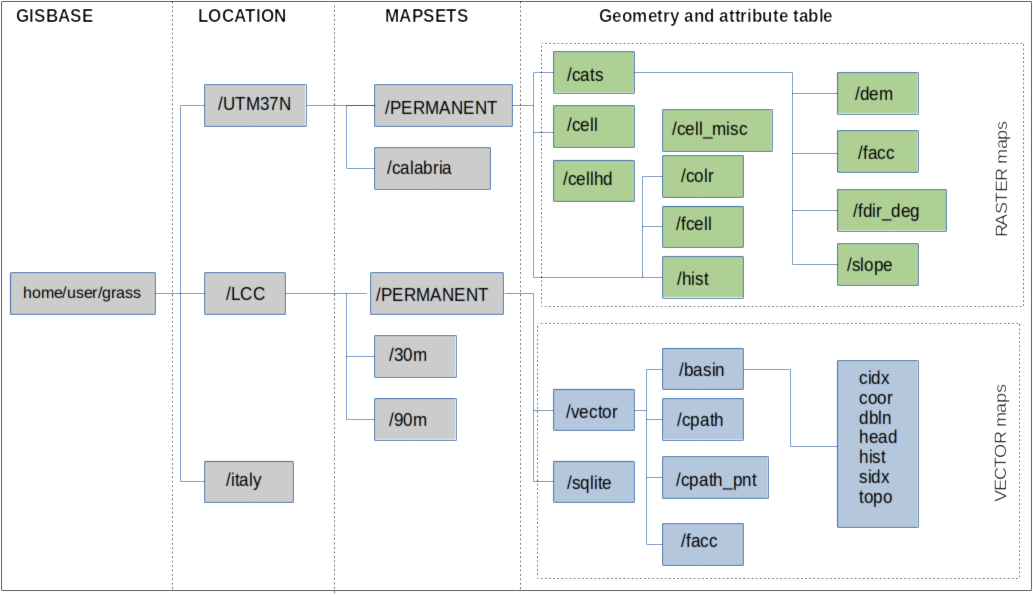
\includegraphics[scale=0.5]{grass_structure}
\caption{Grass internal file structure}
\end{figure}

Time to start your GRASS session – with your GRASS Location and Mapset `PERMANENT’ highlighted click on \emph{`Start your GRASS session'}. GRASS will load up a graphical user interface (GUI) using two windows - a layer manager and the map display. Now you are ready to use GRASS. The following instructions will use the command line interface but this can all be done through the GUI if you prefer this method. 

\section{Importing and displaying GDAL Raster Data}

\subsection*{Importing and extent of DEM}

To import your DEM into GRASS, navigate to the directory containing the DEM files from the command line. 

\begin{lstlisting}[language=bash]
cd destination_folder/dem_grids
r.in.gdal input=dem.tif output=dem
\end{lstlisting}

\noindent To check the regional extent of your raster datset, use:

\begin{lstlisting}[language=bash]
g.region -p

projection: 1 (UTM)
zone:       37
datum:      wgs84
ellipsoid:  wgs84
north:      4213386.67972946
south:      3874847.25407434
west:       134877.89022413
east:       324399.35901918
nsres:      29.13921722
ewres:      29.13921722
rows:       11618
cols:       6504
cells:      75563472

\end{lstlisting}

\noindent You change the region and bring it back to its full extent and original resolution by typing:

\begin{lstlisting}[language=bash]
g.region rast=dem
\end{lstlisting}

\subsection*{Displaying Raster Data}

The GUI interface can be used in the same way as ArcGIS to add and manipulate raster datasets. The following instruction will use the command line, with the advantage of allowing short scripts to create and save map images. It is good practice to check processing steps as you go along, particularly if you are changing the computational region. You can display the raster DEM in a graphical interface from the command line.

\begin{lstlisting}[language=bash]
# Starts display window using monitor wx0
d.mon start=wx0
# Uses a scalable elevation color scheme for the topo map			
r.colors map=dem color=elevation
# Displays the topo map 	
d.rast map=dem
\end{lstlisting}

\subsection*{Creating a hillshaded relief map}

To create a shaded relief map from a DEM, use \emph{r.relief}. Default settings for altitude is 30 degrees above the horizon, azimuth is 270 degrees to the east from north and exaggeration z-scaling factor is set to 1. The map is assigned a grey-scale color table. It is possible to add color to shaded relief maps using r.shade.

\begin{lstlisting}[language=bash]
r.relief input=dem output=dem_shade
\end{lstlisting}

\noindent The elevation dem can be draped and displayed over the shaded relief raster map:

\begin{lstlisting}[language=bash]
d.mon wx0
d.shade shade=dem_shade color=dem
\end{lstlisting}

\noindent It is also possible to combine the shaded relief and dem rasters for output as part of a script (alternatively GMT can be used to display the resulting output). 

\begin{lstlisting}[language=bash]
r.blend first=dem second=dem_shade \ 
	output=colored_shaded_relief percent=40
d.rgb r=colored_shaded_relief.r g=colored_shaded_relief.g \
	b=colored_shaded_relief.b
\end{lstlisting}

\section{Watershed Analysis}

\subsection{Masking to Coastlines}

Before proceeding with hydrological processing of the dem, make sure that you have delineated your region to the desired extent. First clip the dem to coastlines or any other desired shape polygon i.e. country or regional interest. 

\noindent \textbf{GSHSS Coastlines.} High resolution shoreline data can be downloaded from the National Oceanic and Atmospheric Adminstration (\url{www.noaa.gov}). A \textit{.shp} file which will ensure you are using a hierachically arranged closed polygons. Make sure you download Level 1 data which contains continental land masses to ensure you have a complete polygon for masking.

\noindent \textit{Import shapefile}

\noindent Import coastline data to the regional extent of the dem which will be reprojected from lat long to UTM coordinates on the fly.

\begin{lstlisting}[language=bash]
#Import shapefile
v.import input=GSHSS_h_L1.shp output=coast extent=region
#View shapefile 
d.vect map=coast width=2 type=boundary
# Mask dem using shapefile
r.mask vector=coastline
# Display masked dem to check your results 
d.rast dem
#Removing mask
r.mask -r
\end{lstlisting}


\subsection{Filling DEM}

DEM's will have numerous sinks, so before rivers can be extracted, a hydrologically consistent surface needs to be produced. Local depressions will interrupt flow-routing alogorithms and produce incorrect stream networks if incorrect patterns of flow accumulation have been created. However, it is worth noting that not all sinks are errors due to resolution of the data or rounding of elevations to the nearest integer, these sinks can be real-life features. GRASS \emph{r.watershed} module does not require DEM's to be filled. Instead it uses a least-cost search algorithm to traverse the elevation surface to the outlet.

\noindent GRASS \emph{r.fill.dir} module fills DEM's in the same way as ArcGIS's Fill tool available as part of the spatial analyst licence. GRASS follows Henson and Domingue (1998) to filter and fill the elevation map. Using the neighborhood technique, \emph{r.fill.dir} will fill all depressions with one pass across the elevation model and produces a flow direction map by determining slope to each of the 8 surrounding cells (D8 algorithm) and assign a direction. However, in flat areas where cells in a number of different directions have the highest slope, the algorithm will try to find a different route, iterating though this process so it will propogate flow directions from areas where directions are know into areas that can't be resolved. However, be aware that these depression-filling algorithms also create artifical features (e.g. flats leading to parallel streams). 

\begin{lstlisting}[language=bash]
#Sets computational region
g.region raster=dem -p
r.fill.dir input=dem output=dem_fill direction=fdir \
	areas=dem_sinks
\end{lstlisting}

\noindent Use raster calculator to generate a map showing the pixelwise differences between the raw and fill dem:

\begin{lstlisting}[language=bash]
r.mapcalc "dem_diff = dem_fill - dem"
r.colors dem_diff color=differences

# assess univariate statistics of differences
r.univar -e dem_diff

# vectorize filled areas (here all fills are of positive value, see r.univar output)
r.mapcalc "dem_fill_area = if(dem_diff > 0.0, 1, null() )"
r.to.vect input=dem_fill_area output=dem_fill_area type=area

# generate shaded terrain of filled dem for better visibility of results and visualise differences
r.relief input=dem_fill output=dem_fill_shade
d.mon wx0
d.shade shade=dem_fill_shade color=dem_fill
d.vect dem_fill_area type=boundary color=red
\end{lstlisting}

\noindent Grass's \emph{r.fill.dir} module does not deal well with large raster datasets. It is worth exploring python modules \emph{e.g. Richdem} to fill DEMs.

\section{Extracting Stream Network}

\subsection{Enabling Extensions}

Note to use various of the \emph{r.stream.*} tools, it is necessary to use \emph{g.extension} to install the tools as add-ons. This is as simple as \emph{g.extension r.stream.basins}. If you get an error``Please install GRASS development package”, you can install it from the Linux command line using \emph{sudo apt install grass-dev}.

Add-ons installed for this analysis:

\begin{lstlisting}[language=bash]
g.extension r.stream.order \
r.stream.extract \
r.threshold \
r.stream.watersheds \
r.stream.distance \
r.stream.channel \
r.stream.basins
\end{lstlisting}

\subsection{Flow Accumulation}

[The least cost path (LCP) algorithm was originally designed to increase by  Hart et al., 1968 and Ehlschlaeger, 1989 to increase processing speed and reduce the amount of memory consumption. The GRASS module r.watershed starts with potential outlet points normally identified at map boundaries or cells with at least one neighbor with unknown elevation (i.e. masked coastlines).These outlet points are sorted by cost determined by elevation and order in list. The search begins with extracting the cell with lowest elevation (smallest cost) which is removed from the sorted list and marked as processed. Once this is done its neighbors are investigated. Contrary to the downstream costpath, the search proceeds along the least steep uphill slope. At each step during the search, only neighboring
grid cells that are not yet in the search list and not yet processed are added to the list, and drainage direction for these neighboring grid cells is set towards the current grid cell. If a depression is encountered, the search follows the steepest downhill slope to the bottom of a depression and then proceeds again along the least steep uphill slope. The search proceeds in this manner upstream along the least steep slope and terminates when all grid points have been processed. The LCP search provides two results: (a) flow direction for each
cell in a standard D8 manner (O’Callaghan and Mark, 1984), and (b) the order in which cells must be processed for flow accumulation.] [REDRAFT]

The flow accumulation raster can be created using r.watershed using a single flow direction:

\begin{lstlisting}[language=bash]
r.watershed -s ele=dem acc=facc 
\end{lstlisting} 

Problem areas, i.e. those parts of a basin with a likely underestimate of flow accumulation, can be easily identified with e.g.

\begin{lstlisting}[language=bash]
r.mapcalc "problems = if(flow_acc < 0, basin, null())" 
\end{lstlisting} 

\subsection{Stream Network}

Given that modules r.stream.extract and r.watershed produce slightly different vector layers, use r.stream.extract to create a stream network as a vector layer using a basin threshold of 300km${^2}$ which is the equivad.
 
\begin{lstlisting}[language=bash]
r.stream.extract elevation=dem accumulation=facc \
	threshold=300 stream_rast=stream_300 \
	stream_vector=stream_300 direction=fdir
\end{lstlisting}

\subsection{Creating Watersheds}

While r.watershed is able to provide a basins raster outputted, the resulting raster is a series of very small basins. It is possible to use r.basins to identify the main watersheds in the DEM of interest by using the -l flag. 

\begin{lstlisting}[language=bash]
r.stream.basins -l direction=fdir stream_rast=stream_300 \
	basins=basin_300
\end{lstlisting}


\subsection{Extracting Individual Streams for Plotting}

The following example is based on having a list of X Y coordinates for channel heads of interest. This can also be done using a random set of starting points taken from the flow accumulation grid as follows:

\begin{lstlisting}[language=bash]
r.mapcalc "facc_300 = if( "facc" == 300, 1, null())
#v.out.ascii in=facc_300 out=ch.txt format=point layer=-1 separator=',' --o
\end{lstlisting}

It is also necessary to convert the flow direction raster into degrees:

\begin{lstlisting}[language=bash]
r.mapcalc "fdir_deg = if(fdir != 0, 45. * abs(fdir), null())"
\end{lstlisting}

Once we have the coordinates for each of the channel heads in a file, we run \textit{r.path} in a loop to create a vector line layer for each drainage paths (i.e streams). For our purposes, we want to extract point information along the river profile. To achieve this, we create points along the vector map using the resolution of the dem as maximum distance between points using v.to.points. The output vector map has 2 layers - we are interested in layer 2 where each point has its unique category and the distance from the line's start stored as 'along'. To complete river profile information, we use v.what.rast to retrieve values for elevation from the dem and draianage area pixels from the flow accumulation raster and adds those columns to the points file. Now the river data is ready for extraction as an ascii file for further analysis. 

\begin{lstlisting}[language=bash]
i=0
while read X Y; do 
	echo "$X, $Y"
	i=$(( ${i} + 1))
	r.drain input=dem direction=fdir_deg output=cpath_$i \
		drain=cpath_$i start_coordinates=$X,$Y --o 
	v.to.points input=cpath_$i output=cpath_pnt$i \
		use=vertex dmax=30 layer=-1 --o
	v.what.rast cpath_pnt$i raster=dem column=elev layer=2 --o
	v.what.rast cpath_pnt$i raster=facc column=accum_pixels layer=2 --o
	v.db.addcolumn cpath_pnt$i columns="accum_area double" layer=2 --o
	v.db.update cpath_pnt$i column=accum_area \
		query_col="accum_pixels*${SQ_M}" layer=2 --o
	v.db.dropcolumn cpath_pnt$i columns="accum_pixels" layer=2 --o
	v.out.ascii -c input=cpath_pnt$i layer=2 columns=* \
		separator=',' output=riv$i.dat --o
	echo "Created $i stream"
done < ch.txt
\end{lstlisting}

\section{Exporting Files}

Remember for stream network, make sure to specify that the type=line. Areas seem to be automatically picked up with no complaints by GMT when it comes to plotting.

\begin{lstlisting}[language=bash]
v.out.ogr input=vector_file output=vector_file.shp \
	format="OGR_GMT"
\end{lstlisting} 

\section{Useful Commands}

To check the list of rasters or vector files generated during the hydrological analysis, use:

\begin{lstlisting}[language=bash]
g.list raster
g.list vector
\end{lstlisting} 

Another useful tool to check metadata of the raster or vector layer – which will also tell you what tool and criteria you used to generate the raster layer is ‘r.info raster’.

\begin{lstlisting}[language=bash]
r.info rasterfilename
v.info vectorfilename
\end{lstlisting} 






